% !TEX encoding = UTF-8
% !TEX TS-program = pdflatex
% !TEX root = ../tesi.tex

%**************************************************************
\chapter{Resoconto Stage}
\label{cap:resoconto-stage}
%**************************************************************

%**************************************************************
\section{Pianificazione}
\subsection{Pianificazione iniziale}\label{sec:pianificazione-iniziale}
Una prima pianificazione delle attività è stata fatta da me insieme al tutor aziendale, prima dell'inizio dello stage, principalmente definendo e redigendo il piano di lavoro, documento necessario per iniziare lo stage e per avere un'idea delle tempistiche necessarie al completamento degli obiettivi prefissati. Durante lo svolgimento dello stage tuttavia, la pianificazione originaria ha subito delle piccole modifiche, in quanto alcune attività hanno richiesto più tempo di altre. 

\subsection{Sistema di Issue e Gantt}
Per essere sempre entrambi aggiornati sullo stato dei lavori, il mio tutor mi ha suggerito di utilizzare il sistema di issue ampiamente utilizzato in azienda, basato su Redmine. Abbiamo quindi riportato gli obiettivi principali definiti nel piano di lavoro, in modo da tenere traccia di quali sono stati completati e di una stima del tempo richiesto: è infatti possibile segnare una stima delle ore utilizzate per una certa attività. Redmine era inoltre integrato con il git aziendale, permettendo quindi di fare riferimento a specifici commit e di scrivere una wiki relativa al progetto.
\\
Impostando correttamente le date e le priorità tra le attività da svolgere nel Redmine aziendale, era anche possibile generare automaticamente un diagramma Gantt per visualizzare in maniera più semplice informazioni riguardo ogni attività, quali: lo stato, la scadenza e i tempi impiegati, per meglio comprendere i possibili ritardi. Essendo questo un progetto relativamente piccolo tuttavia, la gestione delle ore su Redmine è stata utilizzata poco, ma mi è stata molto utile per imparare come viene gestito un progetto più ampio in azienda.

\subsection{Discussioni e incontri con il tutor}
Soprattutto lavorando principalmente da casa, discutere spesso con il tutor e aggiornarlo sullo stato del progetto e su eventuali dubbi/problemi è stata una parte fondamentale del mio stage. Per questo facevamo una videochiamata al giorno (salvo impegni), per discutere lo stato del lavoro e i prossimi passi da fare. Inoltre, ci incontravamo in ufficio almeno una o due volte a settimana, permettendomi così di mostrargli di persona l'applicazione e fare delle piccole dimostrazioni su cosa era stato fatto e in che modo, ma anche per discutere su come migliorare alcuni dettagli o come risolvere alcuni problemi.

\subsection{Problemi e ritardi}\label{sec:problemi-ritardi}
Come accennato nella sezione \nameref{sec:pianificazione-iniziale} (§\ref{sec:pianificazione-iniziale}) e come vedremo più nel dettaglio tra poco, la pianificazione iniziale ha subito delle piccole modifiche, in quanto alcune attività hanno richiesto più tempo. Questo non è stato un grosso problema perché, viceversa, alcune attività hanno richiesto meno tempo: i problemi principali sono stati nell'utilizzo di CMake e nell'import di un volume DICOM attraverso le librerie aziendali, mentre lo sviluppo della GUI e della pipeline di rendering ha richiesto meno tempo di quanto pianificato.

%**************************************************************
\section{Implementazione}
Vediamo ora nel dettaglio ed in ordine cronologico i passi effettuati durante lo stage per implementare ed utilizzare i concetti discussi nel capitolo 3, utilizzati per sviluppare l'applicazione. Non entrerò nel dettaglio di com'è stata implementata ogni cosa, in quanto il codice appartiene all'azienda.

\subsection{Impostazione ambiente di sviluppo}
La prima settimana era dedicata all'introduzione del progetto: dovevo quindi impostare l'ambiente di sviluppo, discutere con il tutor le modalità di lavoro, gli strumenti, configurare il git aziendale e studiare le librerie che avrei utilizzato, tutti passi preliminari e necessari ad un corretto svolgimento dello stage.
Dopo aver impostato tutti gli strumenti, come Visual Studio con il compilatore corretto, aver installato l'ultima versione di Qt (5.15) e di QtCreator, il primo passo è stato scaricare e studiare le librerie che sarebbero state utilizzate. Ho quindi iniziato con uno studio preliminare di 3D Slicer, per imparare le basi di come importare un volume DICOM, come viene utilizzato il volume rendering e concetti simili, prima di scaricare e analizzare anche VTK. 

\subsection{Studio di 3D Slicer}
Per analizzare al meglio il funzionamento di 3D Slicer, ad inizio stage si era pensato di compilarlo dai sorgenti in modo da poterne effettuare il debug. Tuttavia questo si è rivelato un processo molto arduo, in quanto la documentazione su come compilarlo non era molto precisa, e fare una build completa (con quasi tutti i moduli) ha richiesto anche più di 6 ore su un processore Intel i7 6700k composto da 4 core/8 thread a 4.2Ghz. Dopo qualche tentativo fallito quindi, l'idea è stata abbandonata in quanto non strettamente necessaria. 3D Slicer è stato quindi installato normalmente dal setup disponibile nel sito, ed il suo sorgente è stato sfogliato principalmente attraverso GitHub.

\subsection{Studio e installazione di VTK}
Anche VTK, come ogni libreria, non è perfetta: un problema che purtroppo ho notato subito è che c'è della documentazione molto aggiornata e altra molto datata. Per esempio, cercando su Google:"How to build vtk", uno dei primi risultati è: \href{https://vtk.org/Wiki/VTK/Building/Windows}{vtk.org/Wiki/VTK/Building/Windows}, pagina con ultimo aggiornamento ad Aprile 2014 nel momento in cui questo documento è stato scritto. \'E comunque una documentazione valida per le basi, ma è chiaro che non può essere utilizzata attivamente. Discretamente meglio è la pagina \href{https://vtk.org/Wiki/VTK/Configure_and_Build}{vtk.org/Wiki/VTK/Configure\_and\_Build} , aggiornata al 2017. Avendo già utilizzato CMake in passato, non ho avuto grossa difficoltà a compilare VTK, in quanto è davvero ben gestita e facile da configurare. CMake può essere utilizzato da linea di comando o da interfaccia grafica tramite CMake-gui, applicazione installata insieme a CMake. Per una libreria di queste dimensioni con molte proprietà da configurare, è molto più comodo utilizzare la GUI che permette di visualizzare lo stato di tutte le variabili prima di generare il progetto da compilare, come si può vedere nell'immagine \ref{fig: VTK CMAKE}.

\begin{figure}[h]
    \centering
    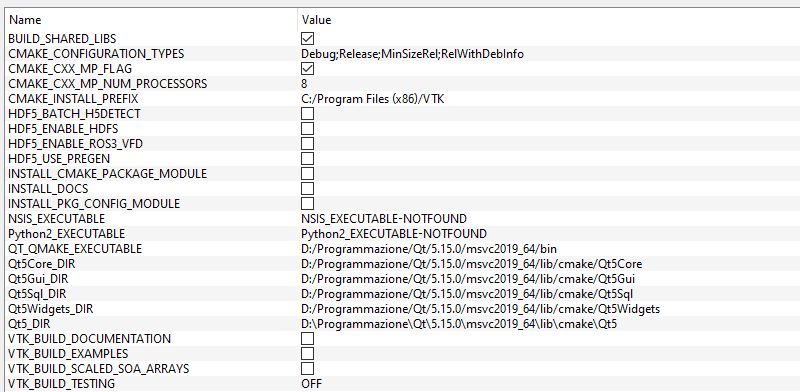
\includegraphics[width=1\textwidth]{immagini/svolgimento/vtkcmake.png}
    \caption{\textit{Alcuni parametri di configurazione di VTK su CMake-gui}}
    \textbf{Fonte}: Stage
    \label{fig: VTK CMAKE}
\end{figure}

A parte qualche dubbio nella compilazione tuttavia, VTK ha un'ottima documentazione sulle classi e offre una ampia gamma di esempi, ed è stato quindi molto interessante ed utile analizzarne i principali per comprenderne il funzionamento e le basi. Oltre agli esempi ufficiali comunque, se ne trovano moltissimi anche su GitHub, grazie al supporto della comunità.

\subsection{Primo CMakeLists}\label{sec:primo-cmake}
Come menzionato nella sezione precedente, avevo esperienza nel fare la compilazione di alcune librerie utilizzando CMake, ma non lo avevo mai utilizzato in un progetto personale. Nel piano di lavoro, CMake era segnato come obiettivo facoltativo con:"F03: porting librerie aziendali su CMake". \'E stato invece deciso con il tutor di iniziare il progetto direttamente utilizzando CMake: innanzitutto per imparare le basi e come utilizzarlo, ma anche per non dover cambiare sistema di build in seguito.
\\
Qt utilizza di default un sistema di build basato su Makefile, generati tramite il comando proprietario qmake su un progetto ".pro". Questo funziona molto bene con Qt, ma è specifico per tale utilizzo. CMake invece è un sistema di build molto più generico e ampiamente utilizzato. L'azienda voleva esplorarne le capacità e le funzionalità, e anche io ero molto interessato ad imparare come utilizzarlo. CMake funziona tramite la scrittura di uno o più file CMakeLists.txt, che definiscono tutti i parametri di configurazione del progetto, le librerie esterne e i file da compilare. Per nostra fortuna Qt ha il supporto a CMake quindi non è complesso da integrare. Diamo un'occhiata ad un semplice CMakeLists.txt di base per Qt.

\inputminted[
frame=lines,
fontsize=\footnotesize,
linenos]{cmake}{capitoli/code/basiccmake.txt}

Analizziamolo per comprenderne i punti principali:
\begin{itemize}
	\item cmake\_minimum\_required: definisce la versione minima di CMake richiesta dal progetto;
	\item project: definisce il nome del progetto e di conseguenza tutte le variabili relative (come per esempio PROJECT\_SOURCE\_DIR);
	\item set: imposta una variabile ad un certo valore, nel nostro caso le variabili CMAKE\_AUTOMOC e CMAKE\_AUTORCC sono variabili utilizzate da Qt, impostate ad ON per specificare di usare il moc e la gestione dei file di risorse;
	\item find\_package: definisce una libreria da trovare ed utilizzare. In caso la posizione di tale libreria non sia nota (per esempio in una variabile di sistema) bisogna passare a CMake il percorso, con una variabile che nel caso di Qt sarà Qt5\_DIR;
	\item add\_executable: definisce l'eseguibile da creare con la relativa lista di file da compilare. In questo esempio anche un file ".ui" e uno ".qrc", file specifici di Qt. Notare che non ci sono i file header ".h" che di norma vengono letti automaticamente, salvo casi particolari;
	\item target\_link\_libraries: definisce le librerie di cui fare il linking nell'eseguibile.
\end{itemize}

\subsection{Ripasso Qt}
Comprese le basi di CMake, dovevo ripassare le funzionalità e la struttura di Qt: avendolo già utilizzato per il progetto di Programmazione ad Oggetti, lo conoscevo già abbastanza bene. Dovevo tuttavia discutere con l'azienda che tipo di interfaccia fare, come strutturare le classi dei widget e come gestire i segnali di click dei bottoni. Ho dovuto quindi progettare e realizzare l'interfaccia di base che sarebbe poi stata utilizzata. Il mio tutor mi ha anche suggerito di utilizzare alcune feature particolari, come la funzione tr() che permette di inserire una stringa che sarà successivamente possibile tradurre in più lingue, ottenendo così un'interfaccia multi-lingua.

\subsection{Integrazione Qt-VTK}
Come accennato nella sezione \nameref{sec:qt-integrazione} (§\ref{sec:qt-integrazione}), VTK è stato compilato con il supporto a Qt, questo offre classi come QVTKOpenGLNativeWidget, da cui è possibile derivare un widget Qt. Un punto molto importante discusso con il tutor aziendale, è stato fare in modo sin da subito che il widget Qt derivato da QVTKOpenGLNativeWidget, che d'ora in poi chiameremo RenderWidget, fosse indipendente: composto quindi dal minor numero possibile di dipendenze, questo per permettere che fosse facilmente trasferibile ad altre applicazioni. Il RenderWidget funzionante si può vedere nella figura \ref{fig: basicwidget}.
\\
Per testare la funzionalità del primo prototipo di RenderWidget, ho cercato degli esempi su GitHub che mostrassero come caricare un semplice modello 3D su VTK, in modo da assicurarmi che funzionasse prima di passare al caricamento di un volume vero e proprio.

\subsection{Volume Mapper}
Come accennato nella sezione \nameref{sec:oggetti-rendering} (§\ref{sec:oggetti-rendering}) e in particolare in \nameref{sec:special-rendering} (§\ref{sec:special-rendering}), un oggetto va visualizzato tramite un vtkMapper. Nel caso del volume rendering, questo può essere fatto utilizzando vtkGPUVolumeRayCastMapper, un mapper che effettua il ray casting sfruttando l'accelerazione hardware della GPU. Questo è il mapper principale che è stato utilizzato, tuttavia in alcuni casi potrebbe non essere disponibile una GPU, è stato quindi deciso di far controllare all'applicazione se è disponibile una GPU sopportata, in caso contrario utilizzerà invece un vtkSmartVolumeMapper: un mapper "intelligente" che supporta varie modalità: di default utilizzerà una GPU se disponibile, altrimenti passerà automaticamente a vtkFixedPointRayCastMapper , un ray caster software (CPU) che chiaramente è notevolmente più lento.

\subsection{Primo prototipo}
Una volta creato e testato il RenderWidget, il primo prototipo di visualizzatore volumetrico è stato fatto caricando le immagini con il loader di VTK, chiamato vtkDICOMImageReader. \'E sufficiente infatti indicargli la cartella da leggere perché provi automaticamente a caricare il volume contenuto in tale cartella, il risultato si può vedere nell'immagine \ref{fig: firstvolume}. \'E importante notare che molti esami TC e RM potrebbero registrare tutte le immagini (e quindi spesso più volumi) in un'unica cartella. In questo caso non è possibile utilizzare vtkDICOMImageReader, che con le impostazioni di default cerca invece di caricare un singolo volume da tutti i file presenti nella cartella selezionata. Nel caso i volumi fossero tutti raggruppati in un'unica cartella, se necessario, si possono separare con vari programmi. In ogni caso, per mia fortuna, il primo esame DICOM fornitomi dall'azienda per effettuare le varie prove era già un singolo volume contenuto in una singola cartella, di conseguenza molto semplice da gestire.

\begin{figure}[h]
    \centering
    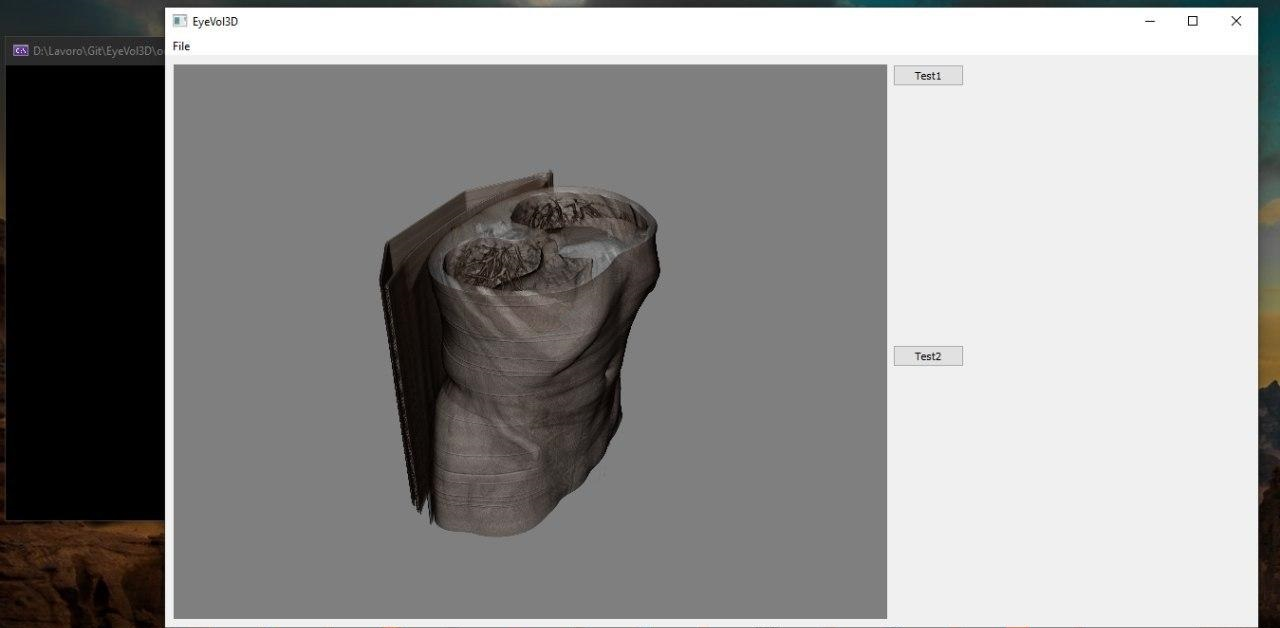
\includegraphics[width=1\textwidth]{immagini/svolgimento/firstvolume.jpg}
    \caption{\textit{Primo volume rendering}}
    \textbf{Fonte}: Stage
    \label{fig: firstvolume}
\end{figure}

\subsection{Strumenti di base - Rotazione}
Ottenuto il primo volume rendering, una delle prime cose essenziali era la possibilità di ruotare la visuale/fare lo zoom e interazioni di base simili. Per nostra fortuna VTK fornisce l'oggetto vtkRenderWindowInteractor che consente di definire un'interazione con la nostra finestra di rendering. Nel nostro caso volevamo una camera che ci consentisse di ruotare attorno al volume utilizzando il mouse, in VTK è chiamata vtkInteractorStyleTrackballCamera. \'E bastato quindi creare un vtkRenderWindowInteractor ed indicargli la finestra di rendering da utilizzare, bisognava inoltre assegnargli un'interazione di tipo vtkInteractorStyleTrackballCamera per ottenere il risultato desiderato.

\subsection{Strumenti di base - Preset}
A questo punto, è stato il momento di aggiungerci i primi strumenti necessari a modificare e meglio visualizzare il volume: il primo e più importante è stato aggiungere la lista di preset, una lista predefinita e standard di funzioni di trasferimento. Come accennato in precedenza, questa è stata presa dal repository di 3D Slicer controllando e rispettandone la licenza. Tuttavia questa lista era in XML, e un XML non è direttamente utilizzabile visto che le funzioni di trasferimento vanno inserite in VTK tramite appositi oggetti. Ho deciso quindi insieme al tutor di fare una piccola libreria designata solo a fare il parsing di tale XML, chiamandola PresetParser. Questa libreria carica l'XML di preset e riempie un array di oggetti generici chiamati VolumePropertyEntry con tutte le proprietà, sarà poi responsabilità dell'applicazione utilizzare questi valori, nel nostro caso caricandoli su VTK. Nel mio programma il parsing fatto all'avvio, caricando la lista dei preset e visualizzando i nomi disponibili, i valori effettivi della funzione vengono caricati in VTK solo quando questo è selezionato, visto che comunque sono pochi e non è un'operazione complessa.
\\
Selezionato un preset quindi, Qt esegue il segnale di "cambio selezione" ed esegue la relativa funzione, che nel mio caso legge la entry del preset e crea gli oggetti di VTK vtkVolumeProperty/vtkPiecewiseFunction/vtkColorTransferFunction, impostandoli poi per il volume corrente.

\subsection{Strumenti di base - Mark}
Mark è il nome che la mia azienda ha dato ad un piccolo omino stilizzato, già utilizzato in alcune loro applicazioni. Mark è molto utile in un contesto tridimensionale, in cui è necessario comprendere l'orientamento di ciò che si sta osservando: immaginate di guardare la TC di una gamba, senza un indicatore di com'è orientata la gamba, ci si potrebbe distrarre e confondere sul sopra/sotto. Come ogni oggetto che viene visualizzato, Mark di base è un vtkActor, di cui è fatto il render tramite un mapper di tipo vtkDataSetMapper. Essendo comune avere un widget che mostra l'orientamento, VTK offre l'oggetto apposito vtkOrientationMarkerWidget, a cui noi assegneremo il nostro vtkActor contenente la mesh di Mark. Una volta caricato si può posizionare in un angolo della finestra e abilitare in maniera simile a come fatto per la vtkInteractorStyleTrackballCamera, il risultato è visibile nella figura \ref{fig: basicwidget}.

\subsection{Strumenti di base - MIP}
Un altro punto molto importante è consentire la possibilità di visualizzare la MIP, questo è stato facile da implementare in quanto VTK offre già dei flag per cambiare modalità di visualizzazione, come possiamo vedere nell'esempio sottostante:
\begin{minted}
[
frame=lines,
fontsize=\footnotesize
]{cpp}
//Max Intensity Proj
vtkVolumeMapper::SetBlendMode(vtkVolumeMapper::MAXIMUM_INTENSITY_BLEND);
//Min Intensity Proj
vtkVolumeMapper::SetBlendMode(vtkVolumeMapper::MINIMUM_INTENSITY_BLEND);
//Default composite
vtkVolumeMapper::SetBlendMode(vtkVolumeMapper::COMPOSITE_BLEND);
\end{minted}

Come si può notare è presente anche la Minimum Intensity Projection, che raramente è utilizzata, ma è stata inserita comunque sotto consiglio del tutor. Com'è intuibile dal nome, funziona come la Maximum Intensity Projection ma utilizzando i valori minimi incontrati lungo il raggio. Nel caso fosse necessario, è immediato aggiungere anche la AVERAGE\_INTENSITY\_BLEND.

\subsection{Strumenti di base - Smoothing}
Lo Smoothing, chiamato anche Jittering, è una funzione che aggiunge un noise alla texture, cercando di rimuovere o ridurre l'effetto di "venatura del legno"(wood-grain effect). Si può notare la differenza nell'immagine \ref{fig: smoothing}, soprattutto nell'ingrandimento. Notare che questa funzione è disponibile solo nel vtkGPUVolumeRayCastMapper, non è infatti disponibile utilizzando il mapper software.

\begin{figure}[h]
    \centering
    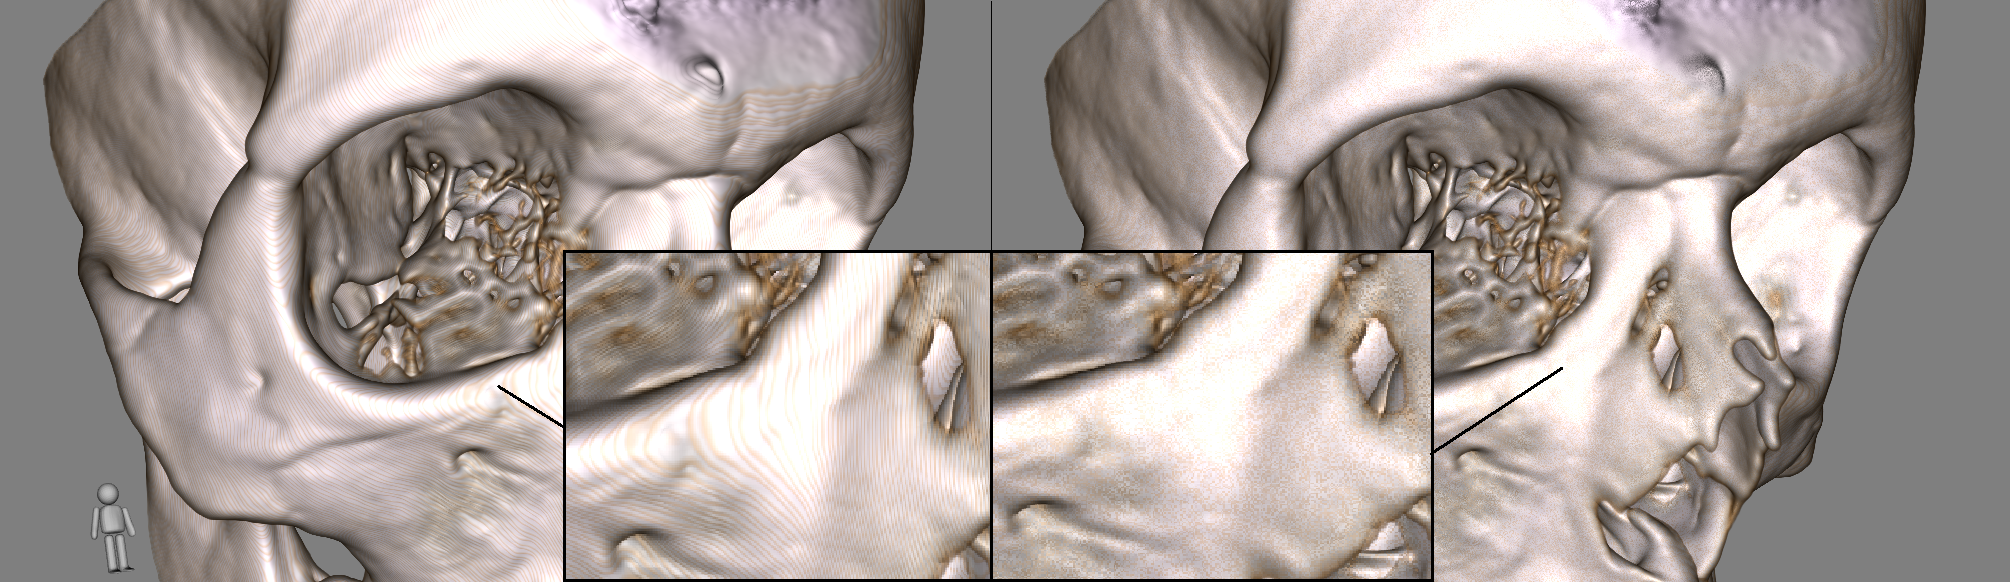
\includegraphics[width=1\textwidth]{immagini/svolgimento/smoothing.png}
    \caption{\textit{Esempio di Smoothing su GPU, OFF a sinistra e ON a destra}}
    \textbf{Fonte}: Stage
    \label{fig: smoothing}
\end{figure}

\begin{figure}[h]
    \centering
    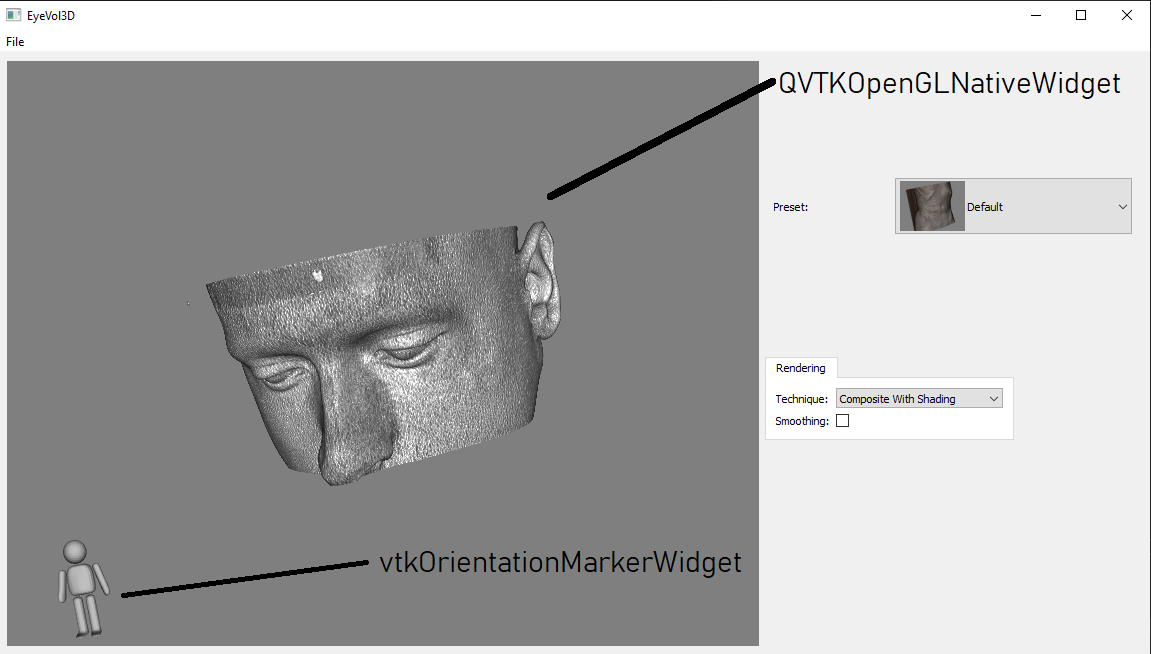
\includegraphics[width=1\textwidth]{immagini/svolgimento/basicwidget.png}
    \caption{\textit{Prima interfaccia con strumenti}}
    \textbf{Fonte}: Stage
    \label{fig: basicwidget}
\end{figure}

\subsection{Strumenti aggiuntivi - Funzione Threshold}
La funzione di Threshold è una funzione binaria per definire una "soglia", in cui a ogni tipo di tessuto da classificare vengono assegnati due numeri: una soglia bassa e una alta. L'altezza del valore massimo dipende dall'opacità, che come si può vedere nella figura \ref{fig: Threshold} si può regolare, il punto alto della funzione quindi avrà lo stesso valore dell'opacità: 0.82 in questo esempio. Affinché un voxel sia considerato rappresentativo di quel tessuto, la sua attenuazione deve rientrare nell'intervallo definito dalle soglie bassa e alta.

\begin{figure}[h]
    \centering
    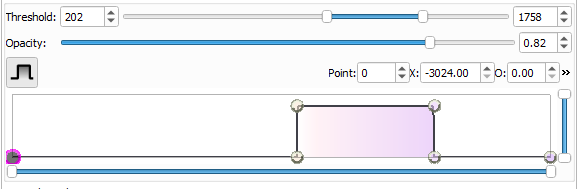
\includegraphics[width=1\textwidth]{immagini/svolgimento/slicerthreshold.png}
    \caption{\textit{Esempio di funzione di Threshold in 3D Slicer}}
    \textbf{Fonte}: Stage
    \label{fig: Threshold}
\end{figure}

Come detto, la funzione di Threshold ha una soglia bassa e una alta, e lo slider che si può vedere nell'immagine ha quindi due puntatori: uno per il minimo e uno per il massimo. Implementare questo non è stato immediato, perché Qt non offre nessun doppio-slider. Ho dovuto quindi cercarne uno che soddisfacesse le mie necessità su GitHub e includerlo nel mio progetto per avere un risultato simile, necessario alla regolazione delle soglie.

\subsection{Strumenti aggiuntivi - Taglio tramite box}
Effettuare il taglio del volume non è stata un'operazione semplice all'inizio: non trovavo esempi coerenti con il mio contesto e molti utilizzavano altri tipi di mapper o cercavano, per esempio, di ridurre la griglia di voxel da mostrare. Dopo un'attenta ricerca nel codice di 3D Slicer e nella documentazione di VTK, mi sono reso conto dell'esistenza del vtkBoxWidget, un widget perfetto per effettuare il tipo di taglio che cercavo. Si crea in maniera molto semplice, e basta assegnargli un vtkProp3D (classe padre di qualsiasi oggetto come vtkActor e vtkVolume) per posizionarlo correttamente su quell'oggetto. Una volta posizionato però, non c'era ancora nessun tipo di conseguenza all'interazione. Ho dovuto quindi creare una callback da collegare al vtkBoxWidget per ricevere ed utilizzare gli eventi di interazione:

\begin{minted}
[
frame=lines,
fontsize=\footnotesize
]{cpp}
class vtkCropBoxChangedCallback : public vtkCommand
{
public:
	void Execute(vtkObject* caller, unsigned long, void*) override;
};
\end{minted}

Questa callback, collegata all'observer vtkCommand::InteractionEvent del vtkBoxWidget riceveva qualsiasi evento di interazione, che ho potuto quindi utilizzare per tagliare il volume. Una volta gestito correttamente il vtkBoxWidget, il taglio effettivo non è stato complesso, in quanto ho trovato che il mapper contiene già un metodo che riceve i 6 estremi da considerare (min/max per x/y/z). Il risultato è visibile nella figura \ref{fig: Taglio Box}.

\begin{figure}[h]
    \centering
    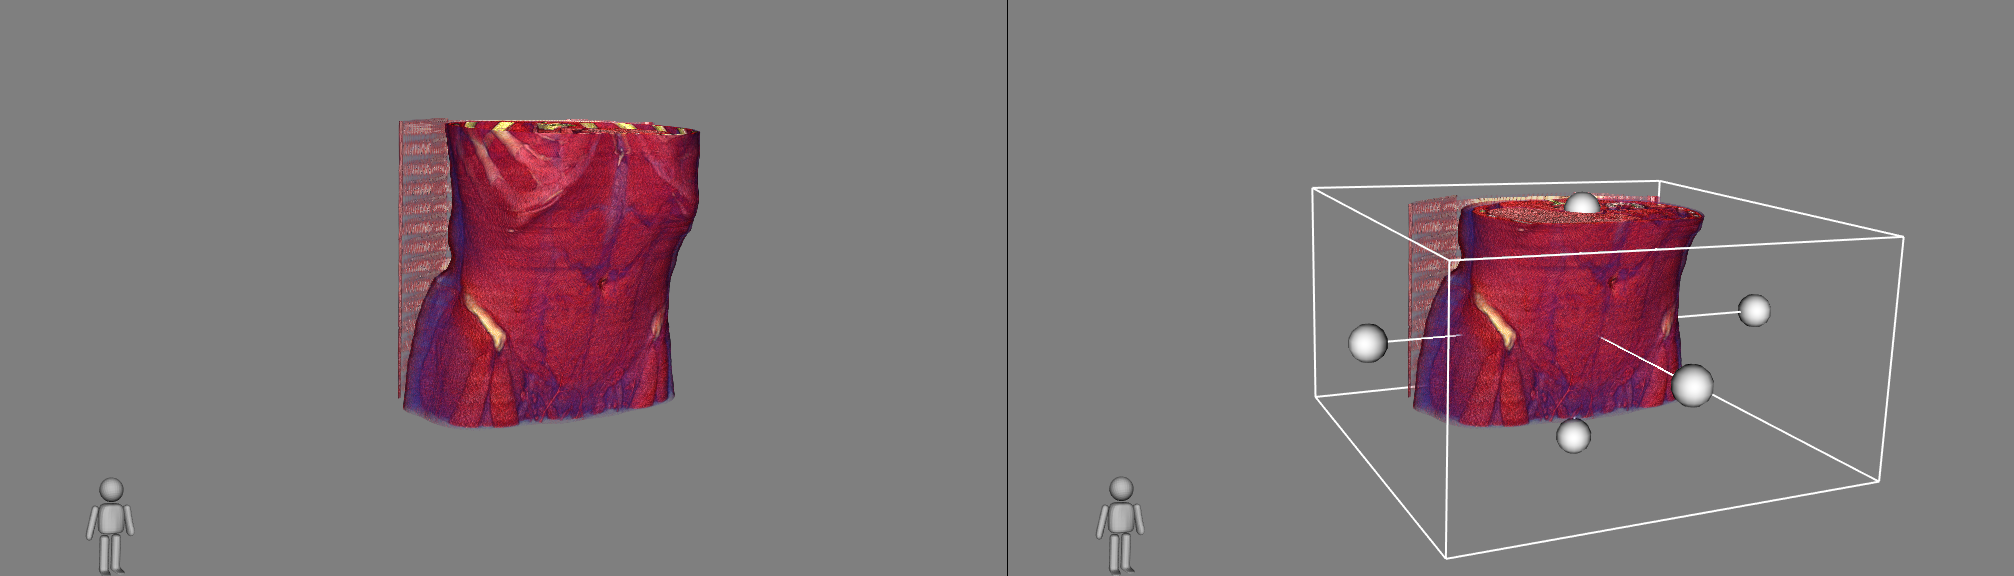
\includegraphics[width=1\textwidth]{immagini/svolgimento/boxcrop.png}
    \caption{\textit{Esempio di taglio del volume tramite vtkBoxWidget}}
    \textbf{Fonte}: Stage
    \label{fig: Taglio Box}
\end{figure}

Notare che, come detto, il metodo di taglio utilizzato con il vtkBoxWidget considera solo il min/max di ogni asse. Questo significa che anche abilitando la rotazione del vtkBoxWidget, questa non consentirà tagli obliqui in quanto considera solo il punto massimo. 

\subsection{Strumenti aggiuntivi - Taglio tramite plane}
Il taglio tramite plane è molto simile al taglio tramite box: si crea il widget vtkPlaneWidget, lo si assegna ad un vtkProp3D e si crea una callback. C'è una differenza importante però: la funzione di taglio di questo tipo è fatta per supportare N piani statici. Questo significa che nel nostro caso con un piano singolo, per spostarlo e aggiornarne la posizione, il piano andrà rimosso dalla lista dei ClippingPlanes e ri-aggiunto ad ogni modifica. Un vantaggio importante però è che un piano di questo tipo consente tagli obliqui in qualsiasi direzione e orientamento. Il risultato è visibile nella figura \ref{fig: Taglio Plane}.

\begin{figure}[h]
    \centering
    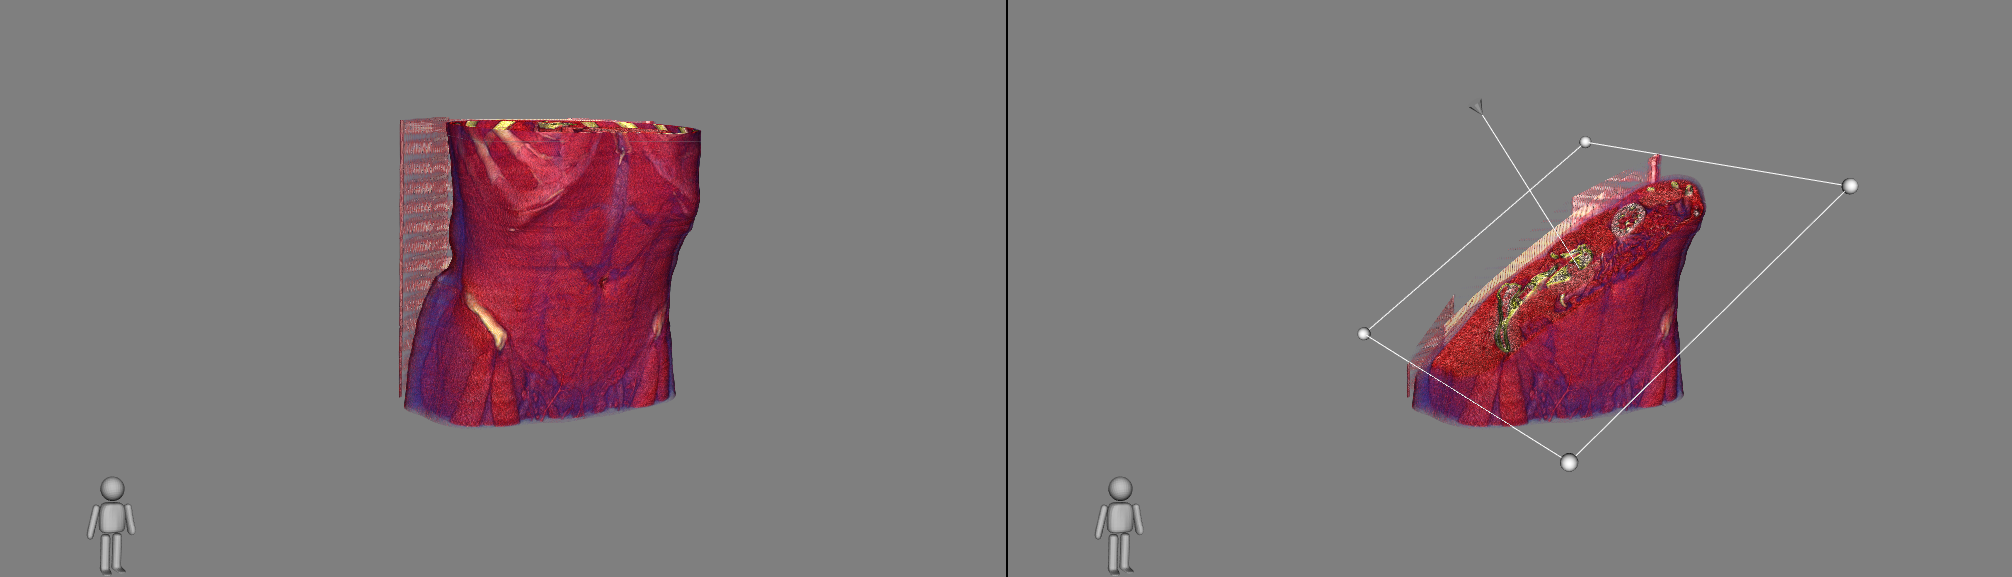
\includegraphics[width=1\textwidth]{immagini/svolgimento/planecrop.png}
    \caption{\textit{Esempio di taglio del volume tramite vtkPlaneWidget}}
    \textbf{Fonte}: Stage
    \label{fig: Taglio Plane}
\end{figure}

Sono anche stati aggiunti metodi e relativi bottoni di utilità nella UI, per reimpostare la posizione/l'orientamento originale del vtkBoxWidget o del vtkPlaneWidget nel caso fosse necessario da parte dell'utente. Si possono anche nascondere: consentendo di tagliare un volume e successivamente nascondere il widget di taglio, così da permettere una visione più pulita del volume.

\subsection{Compilazione librerie aziendali}
Creata tutta la base di visualizzazione e interazione del volume, era importante aggiungere il supporto alle librerie aziendali per l'import di un volume DICOM. Questo richiedeva innanzitutto di portare un considerevole numero di librerie da qmake a CMake, e successivamente di utilizzarle per importare i dati di un volume, che chiaramente andavano convertiti e caricati in VTK.
\\
Questo tipo di dipendenze con CMake è abbastanza facile da gestire, supponiamo di avere una sotto-libreria di una libreria principale, questa si compilerà in maniera simile a quanto visto nel codice nella sezione \nameref{sec:primo-cmake} (§\ref{sec:primo-cmake}), solo che invece di add\_executable su utilizzerà add\_library come segue:

\inputminted[
frame=lines,
fontsize=\footnotesize,
linenos]{cmake}{capitoli/code/sublibrary.txt}

Compilando così una libreria statica il cui nome è sublibrary, da una lista di sorgenti \$\{Sources\}.
La libreria principale che utilizza quella sotto-libreria ora dovrà utilizzare ADD\_SUBDIRECTORY per aggiungere una sotto cartella al sistema di build e compilarne la libreria presente se necessario. A quel punto dopo aver compilato sé stessa dovrà chiamare target\_link\_libraries per dire che la sublibrary è strettamente necessaria e ha quindi bisogno di effettuarne il linking. Nel complesso quindi, saltando comandi come project, si può riassumere così:

\inputminted[
frame=lines,
fontsize=\footnotesize,
linenos]{cmake}{capitoli/code/librarybuild.txt}

Abbiamo così creato una libreria che compila ed include le sue dipendenze. A questo punto il CMake principale che crea l'eseguibile dovrà solo includerla con ADD\_SUBDIRECTORY ed effettuarne il linking con target\_link\_libraries.
\\
Notare che ADD\_SUBDIRECTORY aggiunge solo una subdirectory al sistema di build, cercando il file CMakeLists.txt presente nella cartella indicata. Per aggiungere una cartella di include si utilizza invece l'istruzione TARGET\_INCLUDE\_DIRECTORIES, come nell'esempio seguente:

\inputminted[
frame=lines,
fontsize=\footnotesize
]{cmake}{capitoli/code/targetinclude.txt}

\subsection{Problemi compilazione librerie aziendali}
All'inizio non ho avuto grossi problemi nel portare le librerie su CMake, molte erano relativamente piccole e avevo già scoperto come collegare più CMake tra di loro con la libreria del parser dei preset. Inoltre avendo a disposizione il file di progetto ".pro" per ognuna di esse, era relativamente semplice convertire le istruzioni di compilazione a CMake. 
\\
Tuttavia alcune librerie mi hanno dato grossi problemi, in quanto non riuscivo a compilarle e non riuscivo a comprenderne il motivo. Ne ho discusso con colleghi di lavoro e di università ma nessuno riusciva a comprendere o risolvere il problema. Dopo vari giorni di tentativi, discussioni e ricerche ho scoperto che a quanto pare CMake non voleva l'impostazione che specifica il linguaggio del progetto di tale librerie a C/C\texttt{++}, essendo i file di libreria ".c". Togliendo completamente quell'istruzione tutto ha ripreso a compilare correttamente. Il problema è stato difficile da trovare anche perché tale istruzione andava rimossa da più di una libreria, ma l'errore indicato rendeva difficile comprendere questo dettaglio.

\subsection{Import volume con librerie aziendali}
Una volta riuscito a compilare correttamente tutte le librerie aziendali necessarie al mio progetto, facendo delle prove mi sono reso conto che importare l'immagine dal tipo di oggetto aziendale a VTK era tutt'altro che semplice. Per comodità, sicurezza e per confronto ho lasciato il metodo di import precedente creato tramite vtkDICOMImageReader, e ho fatto l'overload della funzione nella classe del RenderWidget con il nuovo tipo.
\\
Non è stato semplice comprendere come copiare i pixel delle immagini dentro il tipo di VTK, al ché dopo vari tentativi sono andato nel \href{https://discourse.vtk.org/t/trying-to-load-custom-loaded-images-into-vtkimageimport/3704}{forum di VTK (discourse.vtk.org)} per chiedere suggerimenti e consigli su come fare.
\\
Il primo punto da considerare, è se il volume caricato tramite librerie aziendali è composto da immagini a 8, 16 o 32 bit, e da quanti bit di profondità (byte per pixel), queste informazioni vanno considerate per creare correttamente l'oggetto VTK e per calcolare la memoria necessaria. Bisogna anche considerare lo spacing tra le immagini. Letti correttamente questi dati, e compreso come copiare i pixel di ogni immagine dentro un oggetto di tipo vtkImageData, il risultato è subito parso errato, come si può notare nell'immagine \ref{fig: Volume Wrong Order}.

\begin{figure}[h]
    \centering
    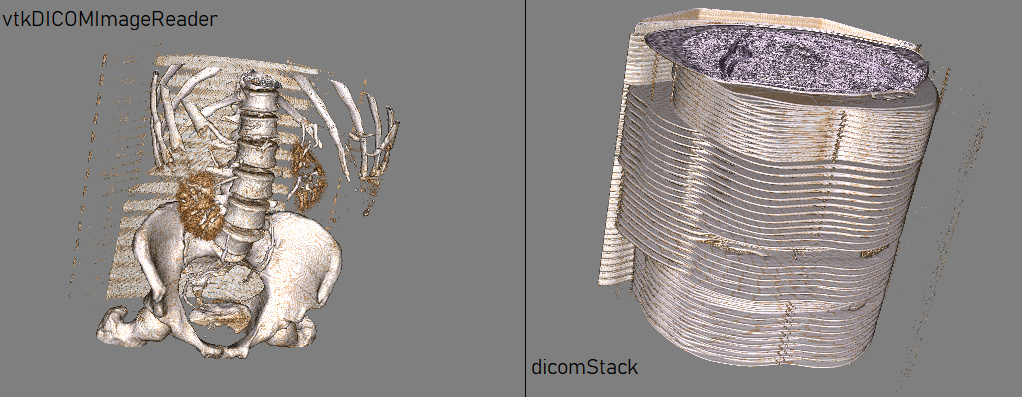
\includegraphics[width=1\textwidth]{immagini/svolgimento/volumebrokenorder.jpg}
    \caption{\textit{Esempio di import volume incorretto (ordine errato)}}
    \textbf{Fonte}: Stage
    \label{fig: Volume Wrong Order}
\end{figure}

Questo perché, come ho scoperto con il tutor, nell'oggetto aziendale che carica le immagini dalla cartella le immagini non sono ordinate, e sono quindi fornite in ordine errato. Per ovviare a questo problema è stato utilizzato un semplice algoritmo di sort per ordinare le immagini correttamente rispetto all'asse Z, documentando che questo andrà migliorato/cambiato in quanto alcune immagini potrebbero andare ordinate rispetto ad un altro asse. Riordinate le immagini il risultato è stato il seguente, visibile nell'immagine \ref{fig: Volume Wrong Scale}. Seppur migliore, è chiaramente errato perché non assomiglia in alcun modo al risultato corretto visibile a sinistra nell'immagine \ref{fig: Volume Wrong Order}.

\begin{figure}[h]
    \centering
    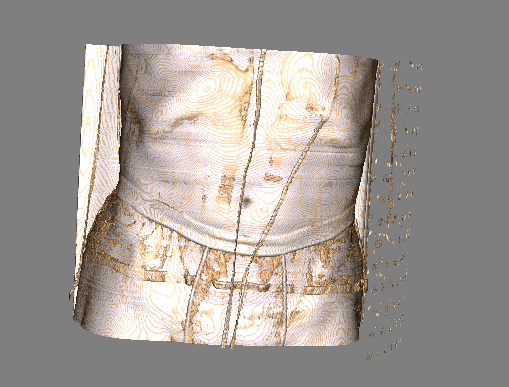
\includegraphics[width=0.6\textwidth]{immagini/svolgimento/volumebrokenscale.jpeg}
    \caption{\textit{Esempio di import volume incorretto (scala errata)}}
    \textbf{Fonte}: Stage
    \label{fig: Volume Wrong Scale}
\end{figure}

Cosa manca? A quanto pare, sempre discutendo nel forum di VTK, ho scoperto che bisogna considerare gli attributi RescaleIntercept e RescaleSlope dell'oggetto DICOM, per scalare correttamente i valori dell'immagine, argomento che anche il tutor mi aveva menzionato. Ho dovuto quindi leggere quei valori, già presenti nell'oggetto aziendale, e considerare questa equazione:
\[ Output units = m *SV + b \]
in cui SV sono i valori memorizzati (stored values) e in cui m è RescaleSlope, quindi anche riscrivibile come: 
\[ Output units = RescaleSlope * x + RescaleIntercept \]
In VTK è stato abbastanza semplice realizzare questo perché è bastato creare un filtro di tipo vtkImageShiftScale fornendogli RescaleIntercept e RescaleSlope, e applicarlo all'immagine. Ottenendo così un risultato corretto.
\\
Tuttavia visto che i casi da considerare sono innumerevoli, i problemi non erano finiti: caricando un'immagine a 12 bit per esempio si presentavano errori del tipo che si può notare nell'immagine \ref{fig: Volume Wrong Value}, in cui il volume è correttamente disegnato, ma è circondato da valori incorretti, rendendo impossibile visualizzarlo.

\begin{figure}[h]
    \centering
    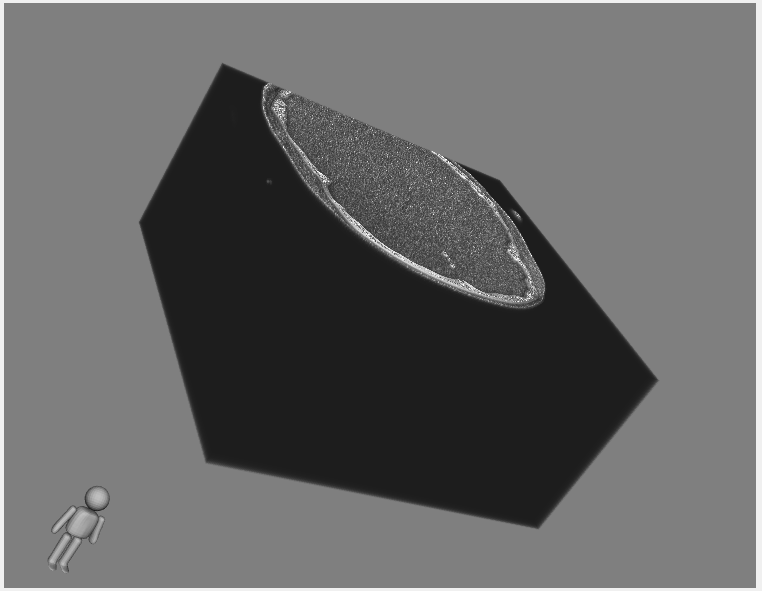
\includegraphics[width=0.6\textwidth]{immagini/svolgimento/volumebroken12bit.png}
    \caption{\textit{Esempio di import volume incorretto (problema con vtkImageShiftScale)}}
    \textbf{Fonte}: Stage
    \label{fig: Volume Wrong Value}
\end{figure}

Questo è un problema legato a vtkImageShiftScale, che di default manda in output valori unsigned, mentre a noi servono valori signed, è stato quindi sufficiente chiamare vtkImageShiftScale::SetOutputScalarTypeToFloat() per indicare di utilizzare valori signed per risolvere il problema.

\subsection{Modifiche interfaccia}
Risolti molti problemi nell'import con le librerie aziendali, il tutor mi ha fatto notare che era meglio migliorare l'interfaccia per renderla più pulita e portatile. Mi ha suggerito quindi di mettere un bottone nel RenderWidget per aprire la schermata di impostazioni, in modo da renderla portatile e meno invasiva. Ho quindi creato un bottone e l'ho posizionato nell'angolo in alto a destra del RenderWidget, cliccarlo apre il pannello di impostazioni come visibile nell'immagine \ref{fig: Final UI}.

\begin{figure}[h]
    \centering
    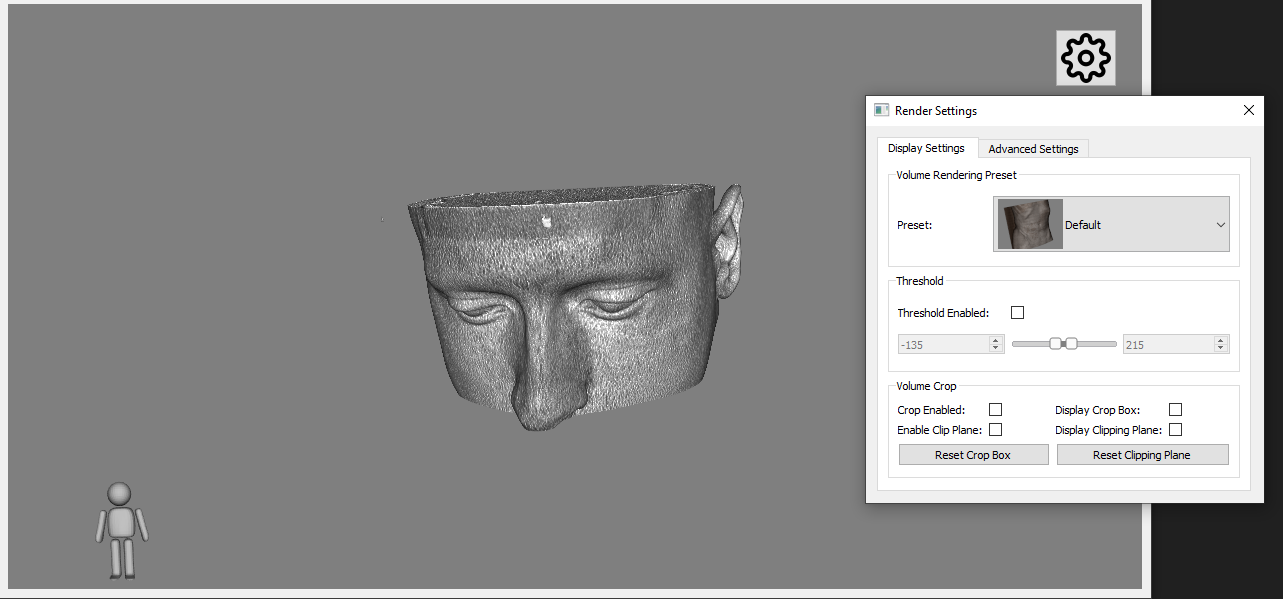
\includegraphics[width=1\textwidth]{immagini/svolgimento/finalnewui.png}
    \caption{\textit{Cattura del design finale della UI}}
    \textbf{Fonte}: Stage
    \label{fig: Final UI}
\end{figure}

Oltre a tutti gli strumenti già discussi in precedenza, nella scheda "Advanced Settings" è presente un tasto per mostrare e volendo cambiare il mapper da CPU/GPU e viceversa in caso sia necessario. Questo permette anche di visualizzare quale mapper è attualmente in uso, per esempio accorgendosi che non è disponibile quello GPU.

\subsection{Esempio porting}
\'E stato anche realizzato un esempio di porting del RenderWidget in un'altra applicazione, sia come test per vedere se era possibile sia per analizzarne il risultato. Nella figura \ref{fig: Porting RenderWidget} si può notare come il RenderWidget sia stato inserito dentro un'altra applicazione. Questa è un'applicazione di demo creta dall'azienda per testare delle funzionalità, e mi è stata fornita per provare ad aggiungere il mio widget nel quarto quadrante, precedentemente inutilizzato.

\begin{figure}[h]
    \centering
    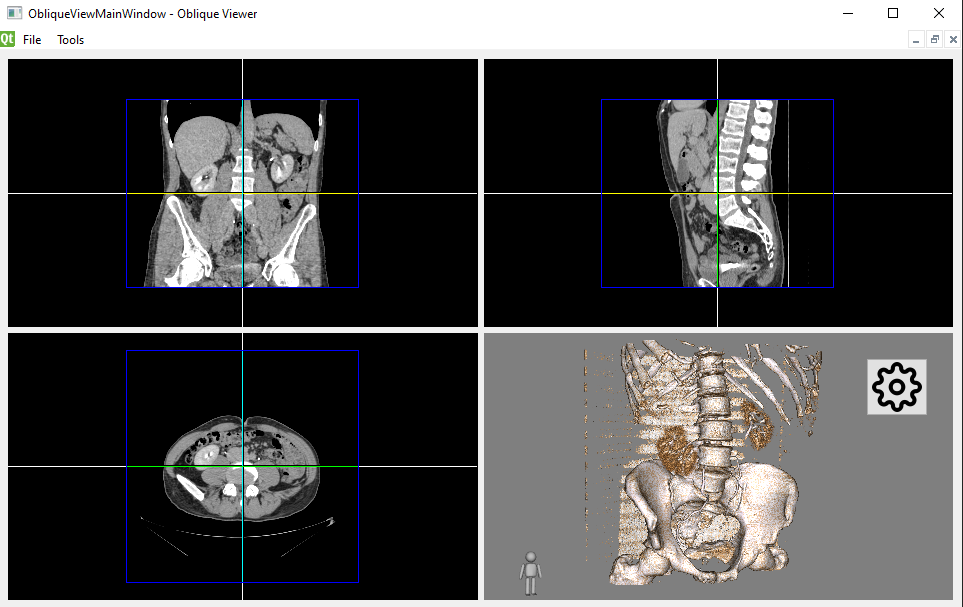
\includegraphics[width=1\textwidth]{immagini/svolgimento/obliqueview.png}
    \caption{\textit{Integrazione RenderWidget in altra applicazione}}
    \textbf{Fonte}: Stage
    \label{fig: Porting RenderWidget}
\end{figure}

Quando viene caricato un volume quindi, sono visibili le immagini sui 3 assi che si possono scorrere, ed il relativo volume. Un possibile sviluppo futuro sarebbe di mostrare nel volume la sezione che si sta osservando sulle immagini, disegnando una linea/un piano sul volume in corrispondenza dell'immagine che si sta osservando, fornendo una visione più precisa, tuttavia questo non era un requisito e non c'è stato il tempo di realizzarlo.

%**************************************************************
\section{Documentazione}
\subsection{Codice}
Il codice è stato propriamente documentato durante la sua scrittura, con commenti nelle funzioni, ma soprattutto nell'header ".h", file interfaccia di C\texttt{++} che contiene solo la definizione di variabili/funzioni e che di solito è il file di riferimento da analizzare quando si utilizza una classe.

\subsection{Wiki}
Un punto essenziale della documentazione, è stato documentare il progetto nella sua interezza nella pagina Wiki disponibile nel Redmine aziendale, lì ho scritto in maniera dettagliata:
\begin{itemize}
\item le istruzioni dettagliate su come compilare il progetto, con la lista di dipendenze e di software necessari;
\item una guida a com'è stato gestito il progetto con CMake e come funzionano i vari CMakeLists;
\item una spiegazione di ogni file di codice prodotto, concentrandomi principalmente su RenderWidget, spiegando come e perché sono state realizzate certe funzioni e come utilizzarle;
\item un esempio di sviluppo futuro, con un esempio documentato di come portare il RenderWidget in un'altra applicazione.
\end{itemize}

%**************************************************************
\section{Test}\label{sec:test-begin}
\subsection{Possibili test su una UI}
Testare un'applicazione con una interfaccia utente non è banale, e dipende molto da come questa è strutturata. Nel caso del corso di Programmazione ad Oggetti per esempio, l'applicazione era realizzata tramite pattern Model-view-controller, questo rende molto semplice testare le tre parti, essendo completamente separate. Nel mio caso non c'era un vero e proprio model, se non quello gestito da VTK, e l'applicazione effettiva era quasi completamente interfaccia grafica. Testare una UI è possibile, si può simulare il click di un bottone, l'inserimento di valori e molto altro, tuttavia quando il risultato è un render come nel nostro caso, verificarne la correttezza in modo automatico diventa un'impresa molto ardua.

\subsection{Test di 3D Slicer e VTK}
Un sistema teoricamente fattibile per testare il risultato del render di un volume discusso con il tutor, è confrontare l'immagine ottenuta tramite render con un'immagine dello stesso volume che si è certi sia corretta per calcolare la differenza: se c'è troppa differenza qualcosa nel render realizzato è incorretto e va corretto. Esplorando i test di VTK, non sembra fare questo nei test del volume, infatti nel codice si trovano commenti del tipo:
\begin{minted}
[
frame=lines,
fontsize=\footnotesize
]{cpp}
// For now we are just checking to make sure that the mapper does not crash.
// Maybe in the future we will do an image comparison.
\end{minted}

Si trovano dei semplici confronti tra immagini, in alcuni test di IO o di filtri semplici, i test del ray tracing e dei volumi si concentrano sul testare il corretto caricamento e funzionamento degli oggetti.
\\
3D Slicer allo stesso modo fa i test principalmente della logica o del funzionamento dei widget simulando click ed eventi, come anche VTK fa in alcuni punti. Occasionalmente salva lo screenshot del risultato del test, o confronta alcuni colori, ma nemmeno in 3D Slicer ho trovato un vero e proprio test per controllare la correttezza di un volume.

\subsection{Test implementati}
Vista l'impossibilità di effettuare un test vero e proprio sul risultato del render del volume, nel tempo che mi rimaneva quindi mi sono concentrato a fare test più utili. Ho quindi studiato ed utilizzato il framework di Qt, chiamato QtTest, per effettuare i test di unità:

\begin{itemize}
	\item un test di unità per la classe che effettua il parsing dell'XML dei preset delle funzioni di trasferimento, in modo da assicurare che i dati letti siano coerenti con quelli nel file per non rischiare la lettura errata dei dati;
	\item un test di unità per il widget "double slider" utilizzato per la funzione di Threshold, in modo anche da imparare come viene testato un widget, simulando l'immissione di valori e la relativa lettura, controllando anche come reagisce cercando di inserire valori incorretti.
\end{itemize}

Una volta realizzati i file cpp dei test, sono stati aggiunti al file CMake del progetto, rendendoli così riconoscibili da QtCreator come test di unità. Questo si effettua aggiungendo add\_test dopo add\_executable, in maniera simile a quanto segue:

\inputminted[
frame=lines,
fontsize=\footnotesize,
linenos]{cmake}{capitoli/code/qttest.txt}

Si può notare come nel target\_link\_libraries del test, oltre a Qt c'è "CustomSlider", l'oggetto dello Slider effettivo da testare, di cui ovviamente il test ha bisogno.